\documentclass[12pt,a4paper]{article}
\usepackage{amsmath}
\usepackage{physics}
\usepackage[]{graphicx} 
\usepackage[left=2.8cm, right=2.8cm, top=1.5cm, bottom=3.5cm]{geometry}
\setlength{\parskip}{0.1cm}

%opening
\title{Quantum Spin Hall Effect}
\author{Chia-Wei Wei}
\date{July 3, 2021}
\begin{document}
\maketitle

\begin{abstract}

The quantum Hall effect is a state with some interesting propeties that the
resistivity is quantized which is in unit of $\frac{e}{2\pi} $ by applying 
the external magnetic field. The spin Hall effect is a effect that 
intrinsic spin of electron would be splited which also caused by external 
magnetic field. But, for quantum spin Hall effect
it is contrast to the 
spin Hall effect with zero charge Hall conductance that the spin Hall 
conductance is quantized that $\sigma^{spin}_{xy}=2$ in unit of  
$\frac{e}{4\pi}$ with the absence of the external magnetic field.
The first proposal of existance of quantum spin Hall
state\cite{PhysRevLett.95.226801} is developed be
Charles Kane and Gene Mele who observe the spin up and down exhibits the 
chiral and  anti-chiral integer quantum Hall effect in model of graphene. 
Then, B. Bernevig and S.C. Zhang\cite{PhysRevLett.96.106802} give the model 
for the quantum spin Hall 
effect. Here we want to show that how quantum spin Hall effect be constructed 
in their paper, the arxiv number of Bernevig and Zhang is 
arXiv:cond-mat/0504147.

\end{abstract}


\section*{Introduction}%
\label{sec:introduction}
\indent
The Bloch Hamiltonian of graphene is a $2\times 2$ matrix which can be
expressed as 

\begin{equation*}
	    {\cal H}({\bf k}) = {\bf h}({\bf k}) \cdot \vec \sigma,
	    \label{dirac}
\end{equation*}

\noindent
where $\vec\sigma = (\sigma_{x},\sigma_{y},\sigma_{z})$ are Pauli matrices
and ${\bf h}({\bf k}) = (h_x({\bf k}),h_y({\bf k}),0)$.  The
combination of inversion ($\cal P$) and time reversal ($\cal T$) symmetry 
requires $h_z({\bf k})=0$ because $\cal P$ takes $h_z({\bf k})$ to 
$-h_z(-{\bf k})$, while $\cal T$ takes $h_z({\bf k})$ to $+h_z(-{\bf
k})$.\\  

In 1988, Duncan Haldane\cite{PhysRevLett.61.2015} proposed the scenario 
for the quantum Hall state
which absence the magnetic field. In his paper, he add a periodic staggered 
local magnetic-flux density $\textbf{\emph{B}(r)}$ in the ${\bf \hat{z}}$
direction normal to the 2D plane, but with $\emph{zero total flux}$ through
the unit cell. The staggerd magnetic field break the time-reversal invariant,
but there is no net magnetic field in this system. 

\begin{equation*}
\begin{split}
  H = &[- t\sum_{\left<i,j\right>}a^{\dagger}_{i}b_{j} + \frac{M}{2}
  \sum_{i=1} (a^{\dagger}_{i}a_{i} - b^{\dagger}_{i}b_{i})] + h.c. + t_{2}\sum_{\left<\left<i,j\right>\right>}[e^{i\varphi}a^{\dagger}_{i}a_{j} +
  e^{-i\varphi}b^{\dagger}_{i}b_{j}] 
\end{split}
\end{equation*}


\begin{figure}[htpb]
  \centering
  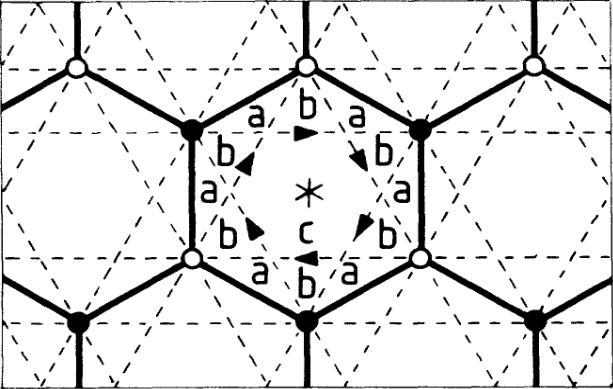
\includegraphics[width=0.6\linewidth]{graphene.png}
  \caption{The honeycomb model showing nearest neighbor hopping (solid lines)
  and second neighbor hopping (dash lines), two sublatices are charaterized
by open and soilid points.}%
  \label{fig:graphene}
\end{figure}

\noindent
where the $t$ and $t_{2}$ are hopping amplitude, the $\varphi$ is the phase
caused by the total fluxes threading through the second hopping.
The third term means that second neighbor hopping term, In his
paper we will see that there is an additional phase which totol flux 
enclose the the second neighbor hopping path would also break the
time-reversal symmetry. The coefficient M in second term represents the 
on-site chemical potential which break the inversion symmetry in the system. 
If we turn on the M term, we can find the gap of Dirac cone is opend. The
Cherm number that we calculate is zero. But, if we consider the magnetic
field is turn on, then we find there is emergent topological property which
Hall conductance is quantized. In other word, there is non-zero Cherm
number appear in this condition. From this point of view, we find that
different symmetry breaking play the different role which open the band gap
and generate the different topological results.
The conclusion of this paper is, while the system is in presence of
magnetic flux, the Chern number is not zero which shows the topological
property which same as the quatun Hall effect system. Haldane calculate the
Hall conductane when system break the time reversal symmetry which is

\begin{equation*}
  \sigma_{H} = \frac{\partial \rho}{\partial B_{z}} \bigg\rvert_{\mu} =
  \frac{\nu e^{2}}{h} \bigg\rvert_{\nu = 1} 
\end{equation*}

\noindent
Haldane proposed the first quantum Hall system without adding the
global magnetic field,that's why quantum anomaly Hall effect be proposed. 
After the several years, in 2005, Kane and Mele considerthe spin-orbital 
coupling base on the Haldan's model. They also found that there also open
the gap at the Dirac point which posses the same non-trivial topological
electric structure. But this kind of topological isulator preserve the time
reversal symmetry which emerge the Quantum spin Hall effect rather than the
Quantum Hall effect.\\ 

The effective Hamiltonian of graphene model at the Dirac points which is\\
\begin{equation*}
{\cal H}_0 = -i\hbar v_F \psi^\dagger(\sigma_x\tau_z\partial_x +
\sigma_y\partial_y)\psi.
\end{equation*}

\noindent
Here $\vec\sigma$ and $\vec\tau$ are Pauli matrices with
$\sigma_z = \pm 1$ describing states on the $A(B)$ sublattice and
$\tau_z = \pm 1$ describing states at the $K(K')$ points. As we know that
if we want to open the gap at the Dirac point, we should add the mass term
in the Hamiltonian.\\ 

In their paper, they stated that we can allow the new term which preserves
the time reversal invariant in this system. The spin-orbital interaction is
allowed which can be described as
\begin{equation*}
{\cal H}_{SO} = \Delta_{so} \psi^\dagger \sigma_z\tau_z s_z \psi.
\end{equation*}

\noindent
where the $s_z$ is Pauli matrix which represents the electron's spin. They
also introduced Rashbe term which break the mirror symmetry
\begin{equation*}
{\cal H}_R = \lambda_R \psi^\dagger (\sigma_x\tau_z s_y - \sigma_y
s_x)\psi.
\end{equation*}

\noindent
For $\lambda_R = 0$, $\Delta_{so}$ there would be opened the gap at the
Dirac point. For $0<\lambda_R<\Delta_{so}$, the energy remain the fintine
until the $\lambda_R$ is graeter than $\Delta_{so}$ whcih energy gap would
be close with quafrafically dispersing bands.\\

Therefore, Kane and Mele found that if system remains the time reversal 
symmetry there would emerges the new topological property in this system.
The effect of spin-orbital interaction is distinct from the ordinary effect
caused by the mass term ($\sigma_z$ or $\sigma_z s_z$). If we consider the
$\sigma_z \tau_z s_z$, we will find that is produce the gaps with the $\it
opposite signs$ at the $K$ and $K'$ points. This kind of special property
prevents that we adiabatically smooth changing from the state generated by
$\sigma_z$ to the state of $\sigma_z\tau_z s_z$. It means that if we want
to change the phase we should close the the gap between the process. If we
consider one spin for $s_z=+1$ or $s_z=-1$, which violet the time reversal
symmetry, is equivalent to the Haldane's model introdcing the periodic
magenetic field with no net flux. If we calculate the Hall conductance, the
result is same as the Haldane's model. So, this system can be seen as two
copies of the Haldane's model but the total Hall conductance is zero for
two opposite sign Hall conductance. Since the spin accumulate in the
opposite gaps for the opposite spin, so electric field will induce the spin
current which is ${\bf J}_s = (\hbar/2e)({\bf J}_\uparrow-{\bf
J}_\downarrow)$ characterized by a quantized spin Hall
conductivity
\begin{equation*}
\sigma^s_{xy}={e\over{2\pi}}.
\end{equation*}

\noindent
As they stated there is come novel phase in this system, if we consider the
Rashba term to break the mirror symmetry we would find the interesting
property in the band structure.
\begin{figure}[htpb]
  \centering
  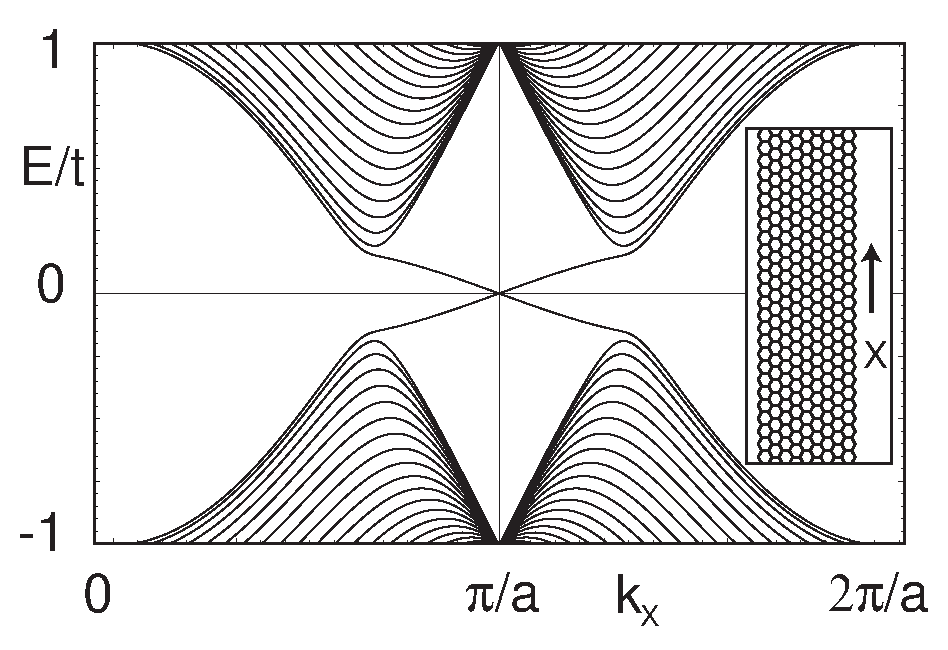
\includegraphics[width=0.6\linewidth]{fig1.eps}
  \caption{In this figure we would see that there is crossing at
  $\pi/a$ which is robust protected by the time revesal symmetry
follows the Kramer theorem.}%
  \label{fig:fig1}
\end{figure}\\

The figure~\ref{fig:fig1} shows that at $k_x$ at $\pi/a$ there is a
degeneracy. 
Kane and Mele had proved that this kind of degeneracy is protected by the time
reversal symmetry which follows the Kramer theorem. It stated that if
system is in time reversal symmetry with half-integer total spin the 
ground state should be at least twofold degeneracy. This is a novel state
of the matter which is distinct from the quatum Hall state.\\ 

Based on the QSHE model of Kane and Mele, Bernevig and Zhang proposed the
another model that realized the QSHE which replaces the electric field in
the spin-orbiral term by the stress strain tensor. However, this kinds of
anology works in this model and they also explained that how to realize
experimentally. In the QSHE system, we want to realized the spin-orbiral 
term which satisfies that $E \sigma_z (xp_y-yp_x)$, we should consider the
particel confined in a two dimensional $xy$ plane, and the electric field
direction should in $xy$ plane as well, the direction spin lies on the $z$
direction. Besides, electric field is not a constant rather than varies
with the $xy$ plane. But, we know that this is difficult to realize
experimentally. So, the scenario of stress strian tensor plays the
important role in the Bernevig and Zhang's model. The following section, I
will show that how deos it do with the strain tensor.

\section*{Method}
In their paper, they use GaAs as the matrial to realize QSHE\@. They stated
that GaAs which is Zinc-blende semiconductors has the point-group symmetry 
$T_d$. According to the this symmetry, the symmetry tensor tensor is
($xy + yx$, etc.) transform in the same way as vector. The shear strain is
symmetry tensor $\epsilon_{ij} = \epsilon_{ji}$ which is equivalent to the 
electric field term in the Hamiltonian:
\begin{equation*} \label{strainelectricfieldanalogy}
\epsilon_{xy} \leftrightarrow E_z;\;\;\; \epsilon_{xz} \leftrightarrow
E_y;\;\;\;\epsilon_{yz} \leftrightarrow E_x
\end{equation*}

\noindent
In this way, we can replace the electric field by the shear strain, the
Hamiltonian can be written as 
\begin{eqnarray*}
& H = \frac{p^2}{2m} + B \operatorname{Tr}{\epsilon} +\frac{1}{2}
\frac{C_3}{\hbar}
[ (\epsilon_{xy} p_y - \epsilon_{xz} p_z) \sigma_x + \nonumber 
& +(\epsilon_{zy} p_z - \epsilon_{xy} p_x) \sigma_y + (\epsilon_{zx}
p_x - \epsilon_{yz} p_y) \sigma_z ]
\end{eqnarray*}

\noindent
Where $\frac{C_3}{\hbar} = 8 \times 10^5 m/s$ for GaAs.\\

From this point of view, we successfully construct the $\it effective$
Hamiltonian for QSHE\@. They presume that the $\Tr \epsilon$ is zero which
would effect the physic of the Hamiltonian. Then, they assume that particles
are confined in the $xy$ plane which means that $p_z$ is zero, and they also
assume that $\epsilon_{xy} = 0$, $\epsilon_{xz}(\leftrightarrow E_y) =g
y$ and $\epsilon_{yz}(\leftrightarrow E_x) = g x$. With this strain
configuration they add the quatum well which is parabolic, the Hamiltonian
which is described above can be expressed as
\begin{equation*}
H= \frac{p_x^2 + p_y^2}{2m} + \frac{1}{2} \frac{C_3}{\hbar}g (y p_x
- x  p_y)\sigma_z + D(x^2 + y^2)
\end{equation*}

\noindent
They make the  change of the variables that
$x \rightarrow (2mD)^{-1/4} x$, $y \rightarrow (2mD)^{-1/4} y$ and $R =
\frac{1}{2} \frac{C_3}{\hbar} \sqrt{\frac{2m}{D}} g$. After the change of
the variabels and let $R = 2$ or $D = D_0\equiv \frac{2mgC_3^@}{16\hbar^2}$
the Hamiltonian would become
\begin{equation*}
  H = \frac{1}{2m} (\vec{p} - e \vec{A} \sigma_z)^2 
\end{equation*}

\noindent
with ${\vec{A} = \frac{m C_3 g}{2 \hbar e}(y, -x, 0)}$.\\

\noindent
The Hamiltonian above which is equivalent to the electon in the magnetic
field but it is charaterize by the spin in the verctor potential term. 
Therefore, we can image that the particle with different spin infleuce by
the different direction magnetic field.
The Hamiltonian in matrix form that can be expressed as 
\begin{eqnarray*}
& H = \left(%
\begin{array}{cc}
  H_{\uparrow} & 0 \\
  0 & H_{\downarrow} \\
\end{array}%
\right) \nonumber\\ & H_{ \downarrow, \uparrow} =
\sqrt{\frac{D}{2m}} [p_x^2 + p_y^2 + x^2+ y^2 \pm R (x p_y - y p_x)]
\end{eqnarray*}

Then the next step, they construct the raising operator and lowering
operator which is simple harmonic oscillator in $xy$ plane. Then, choosing
$z = x + iy$ we have operators for two different spins
\begin{eqnarray*}
& a = \partial_{z^\star} + \frac{z}{2}, \;\;\; a^\dagger = - \partial_z + \frac{z^\star}{2} \nonumber \\
& b = \partial_{z} + \frac{z^\star}{2}, \;\;\; b^\dagger = -
\partial_{z^\star} + \frac{z}{2}
\end{eqnarray*}
\noindent in terms of which the Hamiltonian decouples
\begin{equation*}
H_{\downarrow, \uparrow} =2 \sqrt{\frac{D}{2m}} \left[(1 \m\frac{R}{2} ) a a^\dagger + (1 \pm \frac{R}{2}) b b^\dagger  + 1 \right]
\end{equation*}

\noindent
The eigenvalues of the system can be expressed as 
\begin{equation*}
E^{\downarrow, \uparrow}_{m,n} = \frac{1}{2} \sqrt{\frac{D}{2m}}
\left[(1 \mp \frac{R}{2} ) m + (1 \pm \frac{R}{2}) n + 1 \right] 
\end{equation*}

\noindent
where $aa^\dagger = m$ and $bb^\dagger = n$. In this model, they choose $R
\approx 2$ for which can reduce the Hamiltonian to the oparticle in the
quantum Hall state with one spin. For spin up, Hamiltionian can be
dexcribed by $H_{\uparrow} = \frac{1}{2} \frac{C_3}{\hbar} g 
(2 a a^\dagger + 1) $ with charge Hall conductance which is $e^2/h$. 
For spin down, the Hamiltonian is same as spin up which just replace 
operator $aa^\dagger$ by $bb^\dagger$, but it carries charge Hall 
conductance with minus sign $-e^2/h$. This model can be regarded as two
copies Haldane's model with opposite charge Hall conductance, the total
charge Hall conductance is zero, but two spins experience opposite
direction of $\it effective$ magnetic field, so we get quantized spin
conductance with $2 (e^2/h) (\hbar/2e)= 2(e/4\pi)$ 
which is same as QSHE what Kane and Mele derived.\\ 

Bernevig and Zhang construct the QSHE which replaces the electric field by
the stress strain. In the figrue~\ref{fig:edgecurrent} shows that the
system they proposed is equivalent to a bilayer system; one layer have a
spin up electrons in the presence of a down-magnetic field, the other layer
have spin downs electrons in presence of a up-magnetic field. Because of 
the time reversal invariant, it causes the magnetic is alternative in
different layer.\\ 
\begin{figure}[htpb]
  \centering
  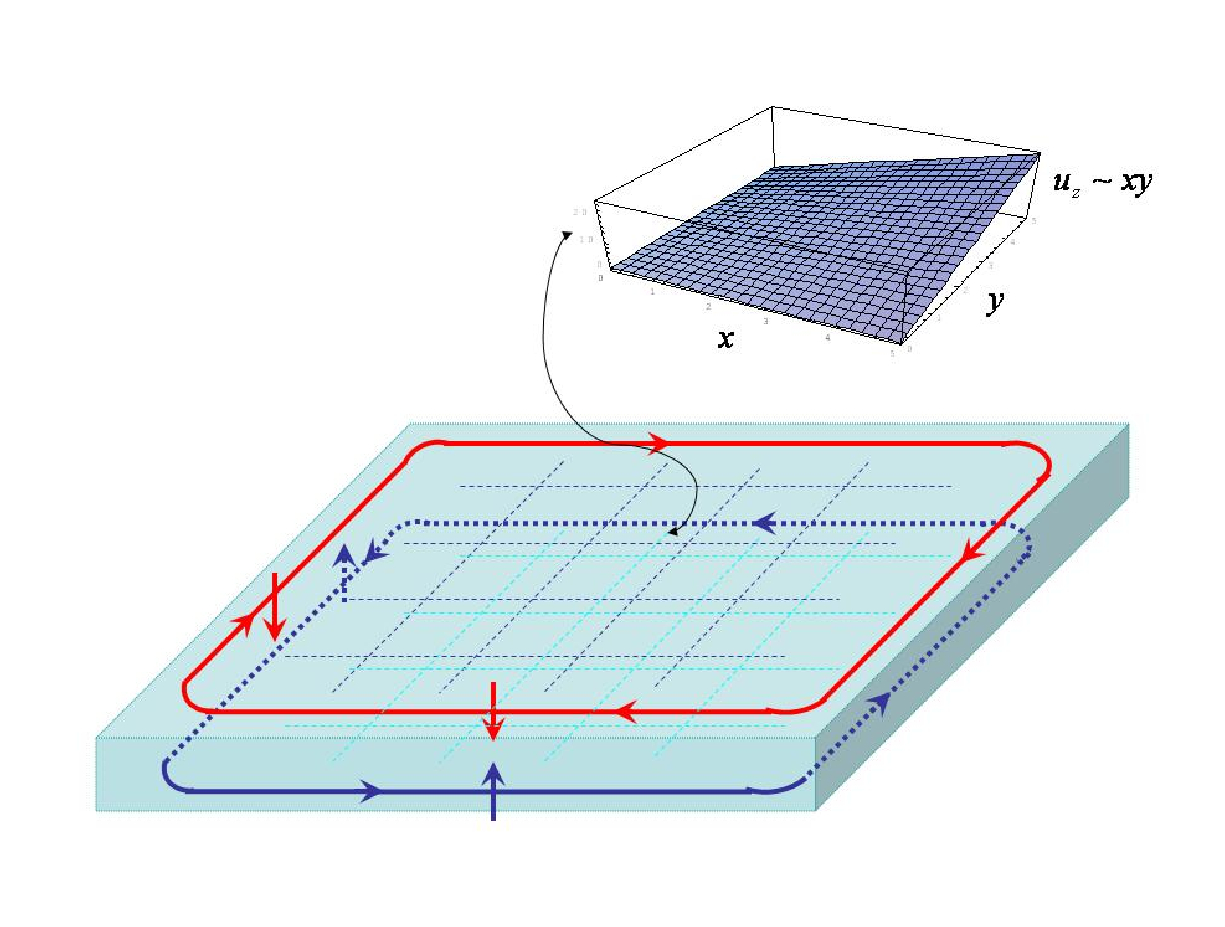
\includegraphics[width=0.6\linewidth]{edgecurrent.eps}
  \caption{Spin up and down electrons have opposite chirality as
they feel the opposite spin-orbit coupling force. Total charge
conductance vanishes but spin conductance is quantized. The inset
shows the lattice displacement leading to the strain
configuration.}
 \label{fig:edgecurrent}
\end{figure}

Then, they discuss how to realized the stress strain tensor form in the
Hamiltonian proposed in their paper. The strain tensor is related to the
diplacement of the lattice atoms from their equilibrium position $u_i$
which can be expressed as $\epsilon_{ij} = (\partial u_i /\partial x_j + 
\partial u_j /\partial x_i)/2$. They choose the equlibrium positions of the
form $\vec{u} = (0,0, 2 g x y)$, then substitutes it into the expression
above that we can get the strain configuration which is same as the form
what they proposed for QSHE($\epsilon_{zx} = g y$ and $\epsilon_{yx} = g
x$). The above discussion can be applied on the GaAs that we pulverize it
on a substate in MBE at a rate which is funciton of the position. The
pulverization rate should vary as $xy$ which is described in the inset of
the fiugure~\ref{fig:edgecurrent}. In this way, they can construct any
kinds of gauge in the magnetic-field language in terms of the different
strain configurations. For Landau gauge, they give a method to realize
which is growing the quantum well in the $[110]$ direction. The strain what
they created for Landau gauge is $\epsilon_{xy} = \frac{1}{4} S_{44} T $,
and $\epsilon_{xz} = \epsilon_{yz} =0$ where $T$ is the impurity
concentration, $S_{44}$ is a material constant and $x,y,z$ are the cubic 
axes. The spin-orbit part of the Hamiltonian is now $\frac{C_3}{\hbar} 
\epsilon_{xy} (p_x \sigma_y - p_y \sigma_x)$. Since they growth in the
$[110]$ direction, they transform to the right coordinate and let
$\epsilon_{xy} = gy' $, the Hamiltonian after the transformation would
become
\begin{equation*}
H = \frac{p^2}{2m} + \frac{C_3}{\hbar} g y' p_{x'} \sigma_{z'} + Dy^2
\end{equation*}

\noindent
This is Landau gauge Hamiltonian that they add the confining term in this
Hamiltonian. Therefore, we can construct any kind of physical gauge what we
want to research by this method. 


\section*{Concolusion}

In this term paper, we introduce Haldane's model which give rise to the
quantum Hall effect with periodic magnetic field and total zero flux
generating in this model. Haldane's find that it can use this model to
describe the quantum Hall state. Then, Kane and Mele proposed the model
which introduce the spin that which doesn't destroy the time reversal
symmetry in the graphene. They found that this is another kind of
topological phase which is different from the quantum Hall state with time
reversal symmetry protecting. After Kane and Mele proposed the QSHE model,
Bernevig and Zhang give a idea that they replace the electric field in spin
orbital coupling term by stress strain tensor, they argue that how to use
this method to derived the same results that what Kane and Mele got in
QSHE\@. They also give the experimental method to realize this method in
lab, they proposed that this method can create any kind of gauge that we
want if we can find the corresponding stress strain tensor.

\bibliographystyle{unsrt}
\bibliography{cm2.bib}





\end{document}
